\documentclass[10pt]{beamer}
\usepackage[absolute,overlay]{textpos}
\usetheme[progressbar=frametitle]{metropolis}
\usepackage{appendixnumberbeamer}
\usepackage[spanish]{babel}
\selectlanguage{spanish}
\usepackage[utf8]{inputenc}
\usepackage{amsmath}
\usepackage[makeroom]{cancel}
\usepackage{booktabs}
\usepackage[scale=2]{ccicons}

\usepackage{caption}
\usepackage{subcaption}
\usepackage{animate} 
\usepackage{amsmath}
\usepackage{bm}
\usepackage{csquotes}
\usepackage{textcomp}
\usepackage{gensymb}
\usepackage{graphicx}
\usepackage[colorinlistoftodos]{todonotes}
\usepackage{hyperref}
\usepackage{fancyhdr}
\usepackage{pdfpages}
\usepackage{attachfile2}
\usepackage{chngcntr}
\usepackage{booktabs}
\usepackage{fancyvrb}
\usepackage{listings}
\usepackage{graphicx}
\usepackage{epstopdf}
% \epstopdfsetup{update}

\usepackage{movie15}
\renewcommand\spanishtablename{Tabla}

\usepackage{pgfplots}
\usepgfplotslibrary{dateplot}

\usepackage{xspace}
\newcommand{\themename}{\textbf{\textsc{metropolis}}\xspace}

\title{Introducción a \textrm{\LaTeX}}
\subtitle{Taller práctico para editar informes y presentaciones}
 \date{\today}
%\date{}
\author{María Luz Stewart -- Patricio Whittingslow}


\begin{document}

\maketitle
\begin{frame}{Agenda}
\begin{itemize}
\item[I.] Presentación - $15$ min
\item[II.] Preguntas? - $5$ min
\item[III.] Practica con ejemplos - $\approx40$ min
\item[IV.] Consultas particulares 
\end{itemize}

\end{frame}
\begin{frame}{Índice}
  \setbeamertemplate{section in toc}[sections numbered]
  \tableofcontents[hideallsubsections]
\end{frame}

\section{Introducción}

\begin{frame}[fragile]{¿Por qué usar LaTeX?}
\begin{itemize}
 \setlength\itemsep{1em}
	
\item Foco en el contenido
\item Automatización de las formalidades de un informe
\item \emph{Facilidad para las ecuaciones!}
\item Gran cantidad de templates online

\end{itemize}
\end{frame}

\section{Ejemplos}

\begin{frame}{Texto}


Para casos en que la geometría y la carga cumplan la condición de axisimetría, es preferible modelar el problema con elementos planos axisimétricos torsionables en vez de elementos tridimensionales.

% Corolario: Los resultados de ambos métodos son totalmente equivalentes en lo que refiere a describir apropiadamente el problema
\end{frame}
\begin{frame}{Presentaciones}
\vspace{0.5cm}

\end{frame}


\begin{frame}{Texto}

Se parte de la deformación en coordenadas cilíndricas y se impone la condicion de axisimetría: $\frac{\partial}{\partial\theta}=0$\\
\vspace{0.6cm}

$\varepsilon_{rr} = u_{r,r}$\\
$\varepsilon_{\theta\theta} = \frac{1}{r}(\cancelto{0}{u_{\theta,\theta}}+ u_{r})$\\
$\varepsilon_{zz} = u_{z,z}$\\
$2\varepsilon_{\theta r} = \frac{1}{r}(\cancelto{0}{u_{r,\theta}}-u_{\theta})+u_{\theta,r}$\\
$2\varepsilon_{rz} = u_{r,z} + u_{z,r} $\\
$2\varepsilon_{z\theta} = u_{\theta,z}+\frac{1}{r}\cancelto{0}{u_{z,\theta}}$\\
\vspace{0.3cm}



\end{frame}


\begin{frame}{Ejemplo - Ecuaciones}
Escribir esto con Word Equation Writer puede llegar a ser muy doloroso o imposible

\hspace{0.45cm}\textbf{Axisimétrico convencional}\hspace{1.2cm}\textbf{Axisimétrico torsionable}

\[
\begin{Bmatrix}
   \varepsilon_{rr} \\
   \varepsilon_{\theta\theta} \\
   \varepsilon_{zz} \\
    \gamma_{rz} \\
\end{Bmatrix}
=
\underbrace{\begin{bmatrix}
   \frac{\partial}{\partial r} & 0 & 0  \\
   \frac{1}{r}    & 0 & 0  \\
   0  & 0 & \frac{\partial}{\partial z}\\
     \frac{\partial}{\partial z} & 0 &\frac{\partial}{\partial r}\\
\end{bmatrix}}_{\left[\partial\right]}
\begin{Bmatrix}
   u_{r} \\
   u_{z} \\
\end{Bmatrix}
\left|
\begin{Bmatrix}
   \varepsilon_{rr} \\
   \varepsilon_{\theta\theta} \\
   \varepsilon_{zz} \\
    \gamma_{rz} \\
     \gamma_{r\theta} \\
      \gamma_{z\theta} \\
\end{Bmatrix}
=
\underbrace{\begin{bmatrix}
   \frac{\partial}{\partial r} & 0 & 0  \\
   \frac{1}{r}    & 0 & 0  \\
   0  & 0 & \frac{\partial}{\partial z}\\
  \frac{\partial}{\partial z} & 0 &\frac{\partial}{\partial r}\\
   0  & \frac{\partial}{\partial r}-\frac{1}{r} & 0\\
     0  & \frac{\partial}{\partial z} & 0\\
\end{bmatrix}}_{\left[ \partial \right]}
\begin{Bmatrix}
   u_{r} \\
   u_{\theta} \\
   u_{z} \\
\end{Bmatrix}\right.
\]	

\end{frame}



\begin{frame}{Ejemplo - Tablas}
\vspace{1cm}
\setlength{\tabcolsep}{20pt}

\linespread{1.2}{
\begin{table}[h!tb]
\centering
\resizebox{0.7\columnwidth}{!}{%
\begin{tabular}{ccccc}
& \multicolumn{4}{c}{Engrane} \\
\cmidrule(lr){2-5}
Coeficiente&\bm{$2$} & \bm{$3$}  & \bm{$4$} &\bm{$5$}  \\ 
\cmidrule(lr){1-1}
\cmidrule(lr){2-5}
\bm{$Y_{j}$}&0,542&0,503&0,55&0,465\\
\bm{$K_{v}$}&0,1189&0,1189&0,0896&0,0896\\
\bm{$K_{h}$}&1,9298&1,9298&1,47&1,47\\
\bm{$Y_{N}$}&0,8761&0,8567&0,8567&0,8269\\
\midrule
% \cmidrule(lr){1-1}
% \cmidrule(lr){2-5}
\bm{$\sigma_{F}$}&26,97&29,06&12,05&14,25\\
\bm{$S_{F}$}&8,62&8.00&19,30&16,31\\
 \bottomrule                    
\end{tabular}}
\caption{Coeficientes de ajuste por flexión}\label{tab:coefBend}
\end{table}}
\end{frame}


\begin{frame}{Animaciones en PDF} 
\vspace{0.9cm}
\begin{figure}

\begin{center}
\animategraphics[autoplay,loop, width=0.8\linewidth]{12}{anim/conejo/a238bc0d367c45aeb93f70ef9650aa74-}{0}{6}
\end{center}
\caption{Animación.}
\label{fig:Conejito}
\end{figure}

\end{frame}
\begin{frame}{ \textsc{ \textrm{Matlab} }}
\begin{figure}

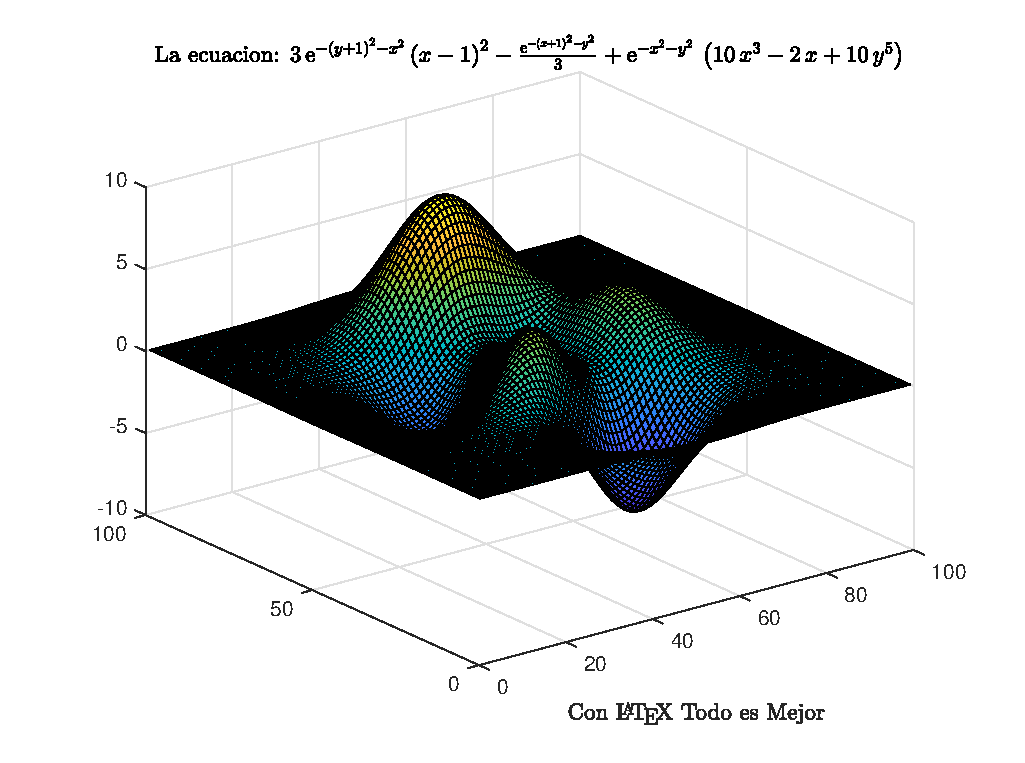
\includegraphics[width=9.6cm]{fig/g6.eps}

 \caption{Hecha con interpretador \textrm{\LaTeX}  en \textrm{\scshape Matlab}}
\end{figure}
\end{frame}

\begin{frame}{Indexing de contenido y referencias}
\vspace{0cm}
\begin{itemize}
\setlength\itemsep{1em}
\item Ecuaciones

\item Tablas

\item Partes, capítulos, secciones, subsecciones etc.

\item Figuras

\item Bibliografía

\end{itemize}

\end{frame}

\section{Comentarios Finales}

\begin{frame}{Limitaciones}

\begin{itemize}
\setlength\itemsep{1em}
\item Fácil de aprender, difícil de amaestrar
\end{itemize}

\end{frame}
\begin{frame}{Gráfico de funciones} 
\vspace{.2cm}
\begin{centering}
\begin{figure}

%La forma de programar en latex es a traves de comandos. Estos inician con barra invertida. (Mencionar algunos de los que estan en pantalla.)
\includegraphics[width=10.6cm]{fig/asme.eps}
\caption{Wordcloud de funciones en un archivo .tex}
\end{figure}
\end{centering}
\end{frame}

\begin{frame}{Gráfico de funciones} 
\vspace{0.2cm}
\begin{figure}
\begin{centering}
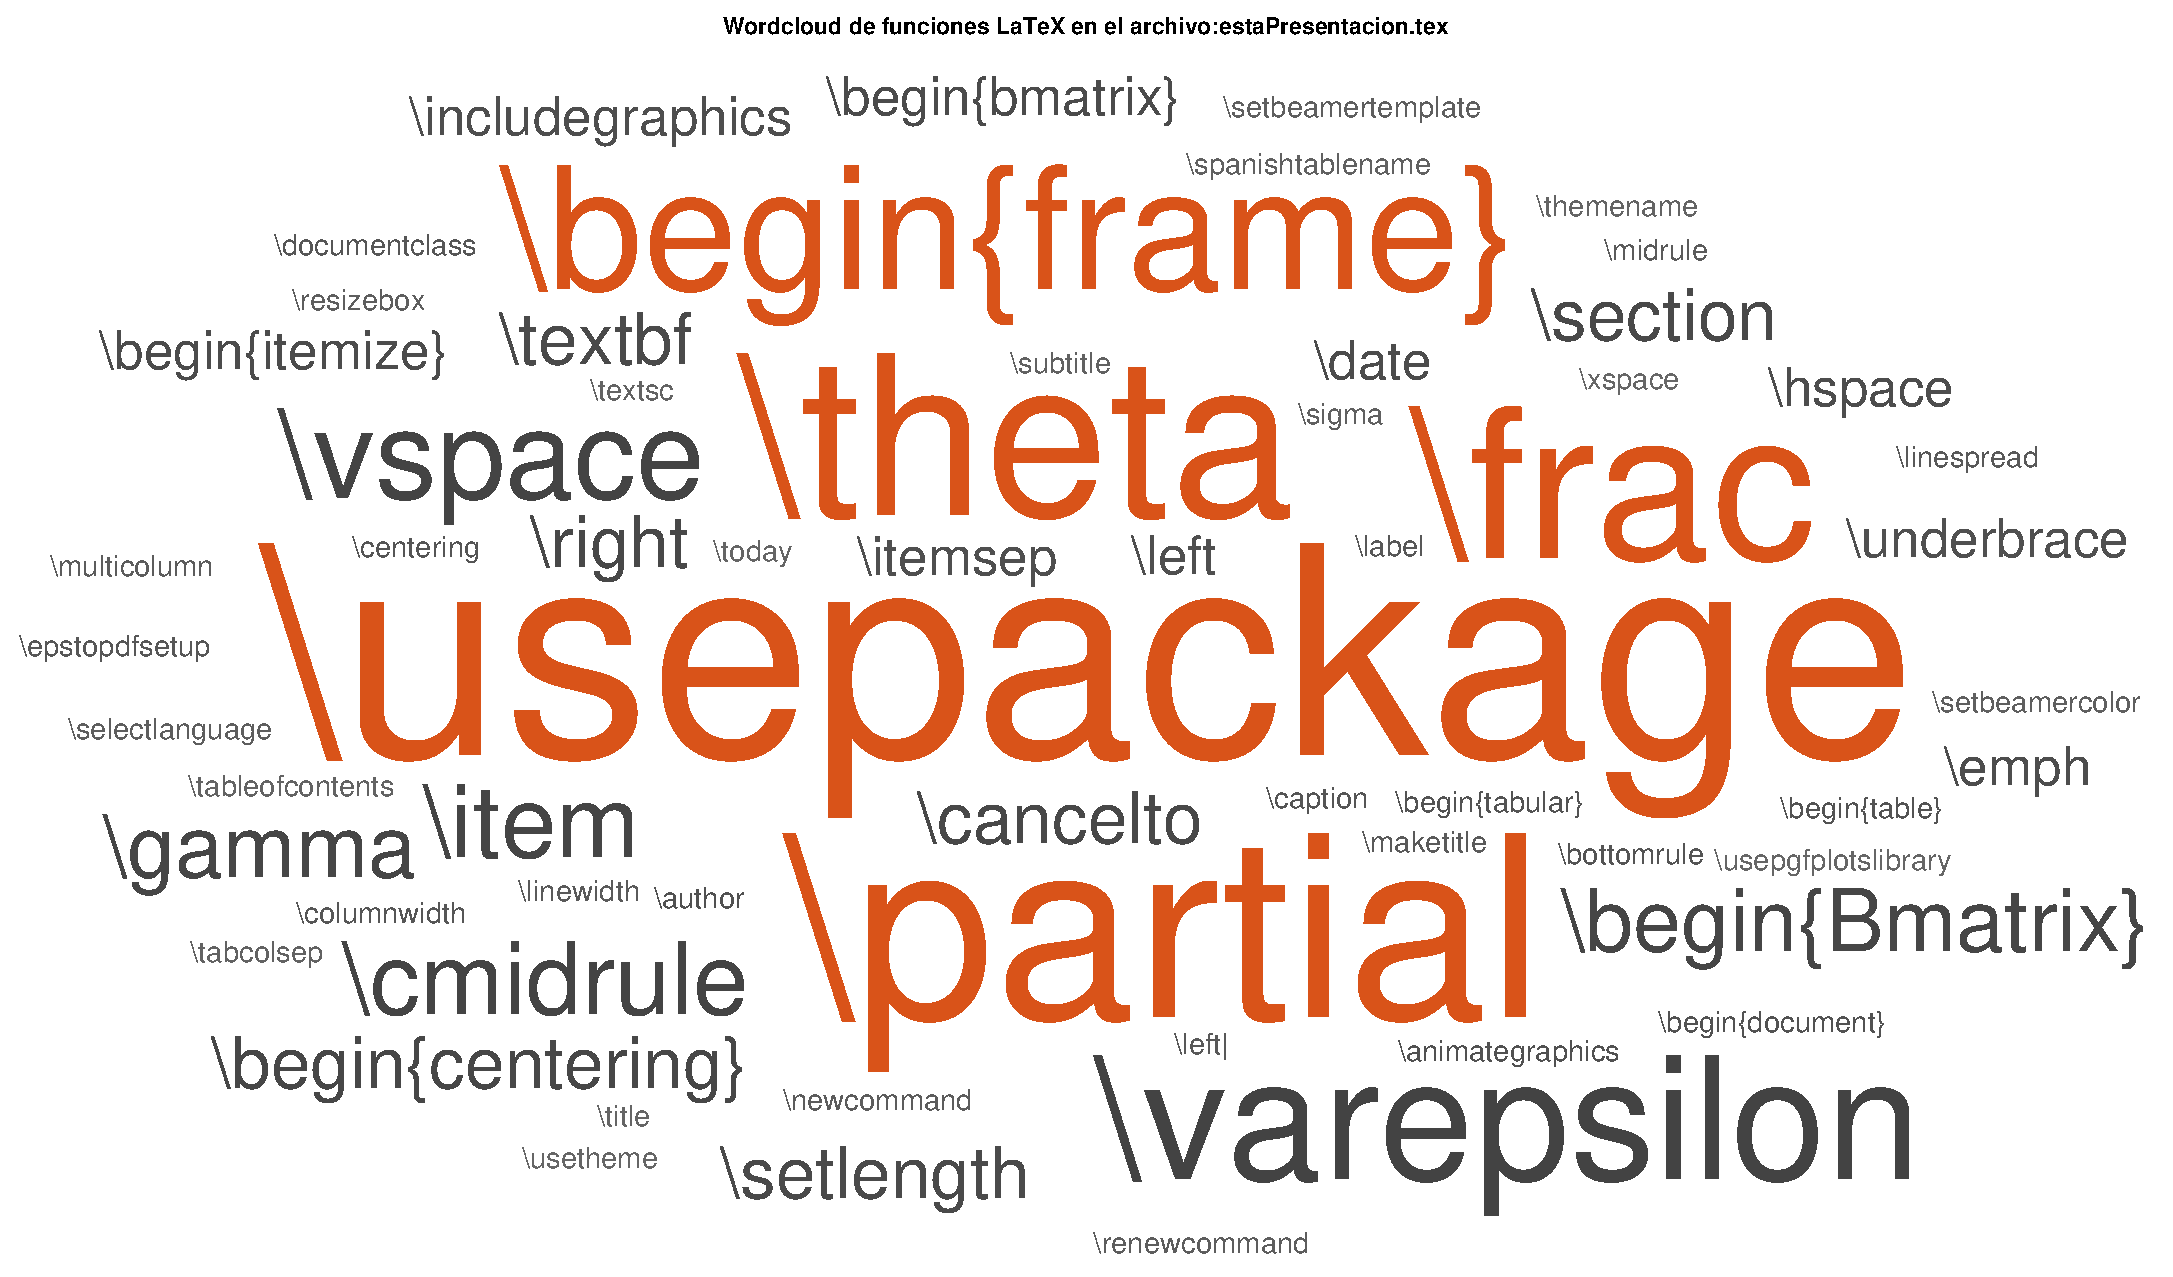
\includegraphics[width=10.6cm]{fig/self.eps}
\caption{Wordcloud de funciones en un archivo .tex}
\end{centering}
\end{figure}
\end{frame}

\begin{frame}{\emph{Física 4}} 
\vspace{0.2cm}
\begin{figure}
\begin{centering}
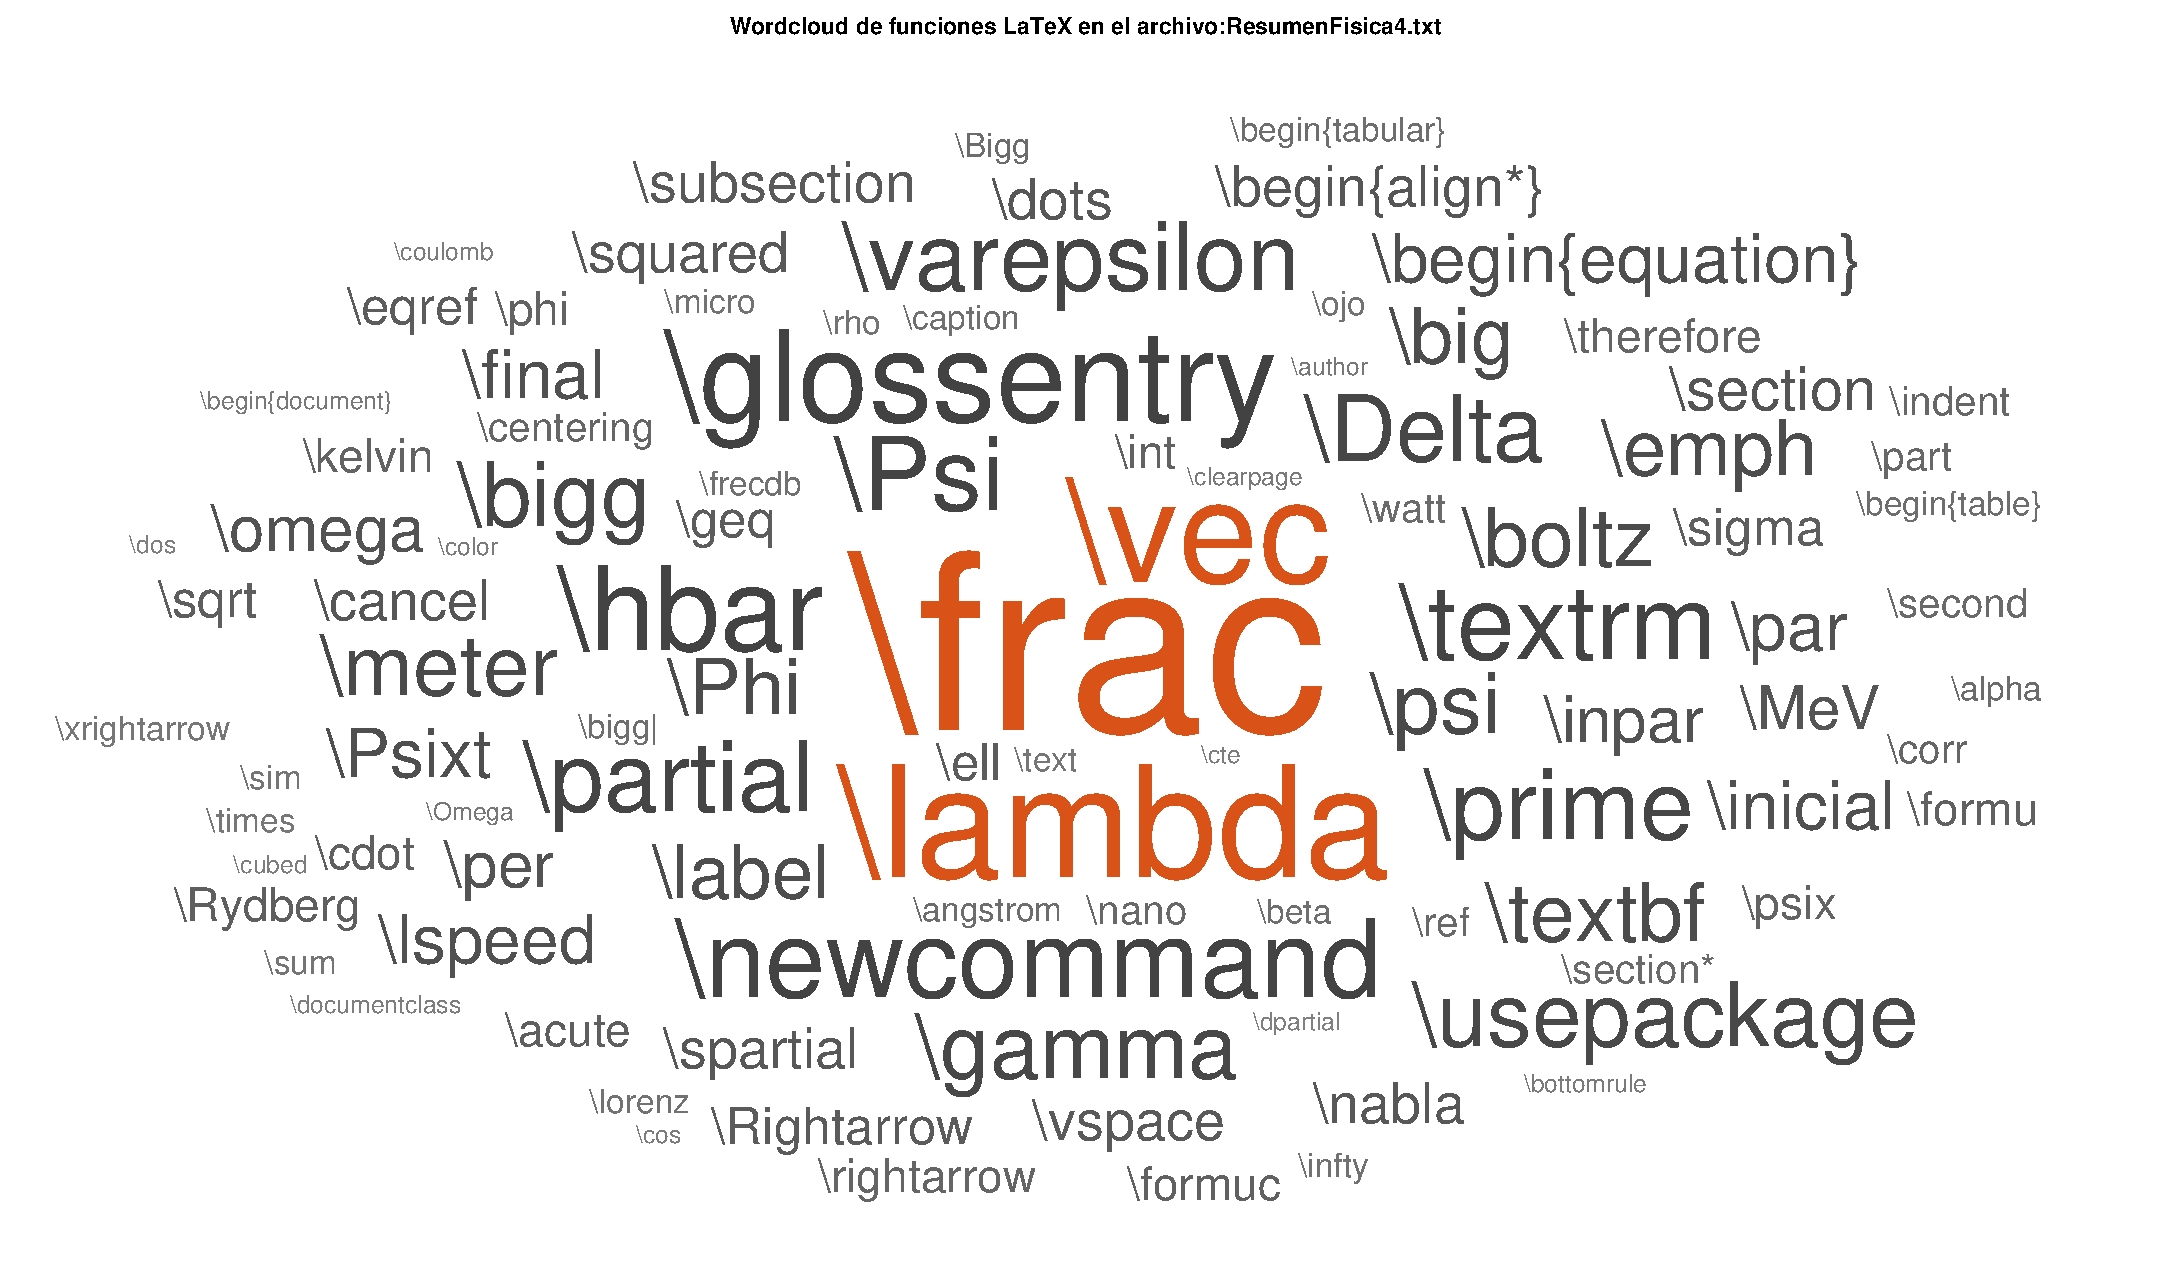
\includegraphics[width=10.6cm]{fig/fisca4.eps}
\caption{Wordcloud de funciones en un archivo .tex}
\end{centering}
\end{figure}
\end{frame}

{\setbeamercolor{palette primary}{fg=black, bg=yellow}
\begin{frame}[standout]
¿Preguntas?
\end{frame}
}


\begin{frame}[fragile]{Sintáxis Comandos}
\begin{block}{Comando}
    \begin{verbatim}
        \comando 
        \comando[parámetros opcionales]{parámetro}
        % asi indico un inline comment
    \end{verbatim}
    \end{block}
Ejemplos de comandos:
\begin{itemize}
    \item \verb|\centering|
    \item \verb|\section{"Nombre de la secci\'on"}|
\end{itemize}
\end{frame}



\begin{frame}[fragile]{Contextos}
\begin{block}{Contexto}
    \begin{verbatim}
    \begin{contexto}
    ...
    \end{contexto}
    \end{verbatim}
\end{block}
Ejemplos de contextos:
\begin{itemize}
    \item \verb|\begin{equation} \end{equation}|
    \item \verb|\begin{document} \end{document}|
\end{itemize}
\end{frame}



\begin{frame}[fragile]{Preámbulo}
    Todo aquello que no esté dentro del contexto \verb|document| es parte del preámbulo. Sirve para definir el formato de la salida. También permite definir y redefinir comandos y contextos.
\end{frame}


\begin{frame}[fragile]{Referencias}
    Se puede hacer referencia a una sección, figura, ecuación, tabla (y muchos más) usando los comandos \verb|ref| y \verb|label|
    
    \begin{block}{Etiqueta}
        \begin{verbatim}
            \label{fig:Conejito}
        \end{verbatim} 
    \end{block}
    \begin{block}{Referencia}
        \begin{verbatim}
            \ref{fig:Conejito}
        \end{verbatim} 
        resulta en el número de la figura: \ref{fig:Conejito}
    \end{block}
\end{frame}
\begin{frame}[fragile]{Listados }
    \begin{block}{Itemize}
        \begin{verbatim}
\begin{itemize}
    \item Algún item
    \item Otro item
\end{itemize}
        \end{verbatim} 
            \begin{itemize}
        \item Algún item
        \item Otro item
    \end{itemize}
    \end{block}
\end{frame}
    \begin{frame}[fragile]{Listados}

    \begin{block}{Enumerate}
        \begin{verbatim}
\begin{enumerate}
    \item Primer item
    \item Segundo item
\end{itemize}
        \end{verbatim} 
            \begin{enumerate}
                \item Primer item
                \item Segundo item
            \end{enumerate}
    \end{block}
\end{frame}


\begin{frame}[fragile]{Bibliografía}
    \begin{block}{Bibliografía}
        \begin{verbatim}
\begin{thebibliography}{9}
    \bibitem{serway}
        Física Moderna, \textit{Raymond A. Serway}
    \bibitem{whitti}
        LaTeX para principiantes con ejemplos, 
        \textit{Patricio Whittingslow}
\end{thebibliography}
        \end{verbatim}
    \end{block}
    \begin{thebibliography}{9}
    \bibitem{serway}
        Física Moderna, \textit{Raymond A. Serway}
    \bibitem{whitti}
        LaTeX para principiantes con ejemplos, 
        \textit{Patricio Whittingslow}
\end{thebibliography}
\end{frame}

\begin{frame}[fragile]{Citar}
    \begin{block}{Cite}
    \begin{verbatim}
Según la fuente \cite{serway}, la velocidad máxima es \( c \). 
    \end{verbatim}
    \end{block}
    Según la fuente \cite{serway}, la velocidad máxima es \( c \). .
    
\end{frame}

\begin{frame}{Escritura de texto}
    \begin{itemize}
    \item Un solo enter no tiene ning\'un efecto.
    \item Una l\'inea vac\'ia, o \texttt{\textbackslash par}, separa p\'arrafos.
    \item \texttt{\textbackslash newline} y \texttt{\textbackslash\textbackslash } generan una nueva l\'inea sin separar p\'arrafos.
    \item Se ignoran los espacios y enters de m\'as.
    \item Los caracteres especiales (\%, \&, \$, \textbackslash, etc) tienen comandos espec\'ificos si quieren imprimirse.
    \item En muchos casos se ignoran los espacios despu\'es de un comando. Esto se puede solucionar agregando \texttt{\{\}} inmediatamente despu\'es.
    \item Si us\'as el layout del teclado en ingl\'es, las tildes se pueden escribir m\'as c\'omodamente con \texttt{\textbackslash 'a}, y la e\~ne con \texttt{\textbackslash}$\sim$\texttt{n}.
\end{itemize}
\end{frame}


\begin{frame}[fragile]{Jerarquía de contenido}
    El contenido puede ordenarse jerárquicamente en secciones, subsecciones, y subsubsecciones mediante los siguientes comandos: 
    \begin{verbatim}
        \section{Nombre sección}
        \subsection{Nombre subsección} 
        \subsubsection{Nombre subsubsección}
    \end{verbatim}

\end{frame}

\begin{frame}{Modo matemático}
\begin{enumerate}
    \item Inline: \texttt{\textbackslash ( x=4 \textbackslash )} 
    \item Display: \texttt{\textbackslash [ x=4 \textbackslash ]} 
    \item Ecuaci\'on numerada: \texttt{\textbackslash begin\{equation\}  x=4 \textbackslash end\{equation\}} 
\end{enumerate}
    La mayor\'ia de los comandos matem\'aticos no son v\'alidos fuera de estos contextos (por ejemplo, las letras griegas). Si bien algunos son nativos de \LaTeX, es conveniente siempre incluir las librer\'ias amsmath, amsfonts y amssymb. 
    
Para encontrar símbolos:
\begin{itemize}
    \item http://detexify.kirelabs.org/classify.html 
    \item mathpix
\end{itemize}
\end{frame}


\end{document}

